\documentclass[UTF8,11pt]{ctexart}
\usepackage[a4paper,margin=2.3cm]{geometry}
\usepackage{amsmath,amssymb,amsthm}
\usepackage{booktabs}
\usepackage{graphicx}
\usepackage{float}
\usepackage[numbers]{natbib}
\usepackage{hyperref}
\usepackage{xcolor}
\usepackage{enumitem}
\usepackage{array}
\usepackage{longtable}
\usepackage{caption}
\graphicspath{{figures/}{./}}
\hypersetup{colorlinks=true,linkcolor=blue,citecolor=blue,urlcolor=blue}
\captionsetup{font=small}
\newcounter{algobox}
\renewcommand{\thealgobox}{\arabic{algobox}}
\newcommand{\algcaption}[1]{\refstepcounter{algobox}\caption*{\textbf{算法\thealgobox：}#1}}

\newtheorem{proposition}{命题}
\newtheorem{remark}{评注}
\newtheorem{assumption}{假设}
\newtheorem{definition}{定义}
\newcommand{\qos}{q}
\newcommand{\T}{\mathcal{T}}
\newcommand{\J}{\mathcal{J}}
\newcommand{\N}{\mathcal{N}}
\newcommand{\A}{\mathcal{A}}
\newcommand{\D}{D}
\newcommand{\U}{U}
\newcommand{\w}{\boldsymbol{w}}
\newcommand{\p}{\boldsymbol{p}}
\newcommand{\g}{\boldsymbol{g}}

\title{\textbf{面向Token推理服务的三层嵌套固定点候选响应框架：\\
平台--中间商--用户结构下的批发价格、容量分配与QoS反馈\\
\large（修订版：修正需求口径与外部选项，2026-06-18）}}
\author{匿名作者}
\date{\today}

\begin{document}
\maketitle

\begin{abstract}
大模型推理服务的负载时段性波动强，高峰时段过量请求会导致GPU拥塞和QoS退化。本文面向平台--中间商--用户三层推理服务市场，提出一个\textbf{算法诱导嵌套固定点候选响应系统（Algorithm-Induced Nested Fixed-Point Candidate Response System, AINF-CRS）}：平台在有限候选集合内排序分时批发价，中间商通过约束优化求解器非合作地确定零售价与跨时段容量分配，用户按含外部退出选项的logit随机效用模型在中间商、时段之间以及退出之间迁移，需求与QoS经阻尼固定点迭代内嵌于每次利润评估。该系统的定位不是连续策略空间中的全局均衡证书，而是给定求解器路径下的可复核策略筛选工具。理论层面，用户层证明有限拥塞博弈的纯策略Nash均衡存在（微观基础），并给出logit SUE--QoS固定点的存在性和压缩条件下的收敛判据（计算稳定性）；中上层采用\textbf{算法诱导候选稳定性}，以给定求解器搜索半径内是否存在显著单边偏离作为候选稳定性判据。

\textbf{本修订版的核心更正。} 相对于早期版本，本版修正了两处会显著改变定量结论的建模缺陷：（一）刚性/重放需求此前对每个中间商都乘以整个时段的总选择份额，导致总需求随中间商数量$J$近似线性放大；本版改为按渠道自身份额分配，使每时段刚性到达量与$J$无关。（二）用户离散选择此前在全部内部$(j,t)$选项上归一化、缺少no-purchase外部选项，导致利润评估与“退出概率”诊断处于两个互斥模型；本版加入显式外部退出选项，使利润、用户inclusive value和退出概率在同一模型内自洽。所有数值实验在修正后重跑。

\textbf{修正后的主要发现（均为重跑真实值）。} 在原始合成需求水平（$\rho=1.0$）下，市场并不拥塞（峰值利用率约0.81--0.85），因此QoS感知定价相对忽略QoS的动态定价仅带来$+0.32\%$系统利润差异；这说明早期版本报告的$+13.61\%$增益主要来自需求口径放大将利用率推高至0.91以上的人为效应。但需求规模扫描显示，QoS感知的价值是\textbf{条件性的}：当需求规模上升到$\rho=1.3$--$2.0$、利用率真正逼近容量边界时，QoS感知相对无QoS动态定价重新获得$+9.3\%$至$+14.5\%$的真实系统利润改善，并将最低QoS从0.76--0.90恢复到1.0000。在加入外部退出选项的自洽模型中，无约束收入最大化的平均零售价被内生约束在1.07附近（因继续涨价会触发用户退出），用户inclusive value保持正值（$+1.57$）；而零售价不超过0.80的价格保护合约同时提高了平台收入（从1501提高到1921）、提升inclusive value（从1.57到2.28）并降低退出概率（从20.7\%到10.2\%），形成可解释的双赢区域。机制归因表明，核心驱动是\textbf{将拥塞风险内化到中间商决策}，而非依赖特定QoS函数形式。本文结论严格限定在合成参数、单平台结构、求解器路径和候选搜索精度之内：AINF-CRS的现实定位是离线机制仿真与策略筛选工具，上线决策仍需真实需求校准和trace-driven验证。
\end{abstract}

\noindent\textbf{关键词：}推理服务；Token定价；中间商；嵌套固定点仿真；算法诱导候选响应；跨时段容量分配；QoS反馈；外部退出选项；机制诊断

% ============================================================
\section*{修订说明（审稿回应）}
\label{sec:revision_note}

本版是对早期稿件的实质性修订，集中修复了审稿过程中识别出的建模与实现缺陷，并据此重跑全部实验。为便于核对，先在此集中列出修订内容；正文相应位置另有详细讨论。

\begin{enumerate}[leftmargin=2em]
  \item \textbf{需求口径修正（最关键）。} 早期版本式中刚性/重放需求项写作$\bar R_t\,\sigma[\beta(v_r-p_{j,t})]\sum_{k}s_{k,t}$，即每个中间商$j$都乘以整个时段的总选择份额$\sum_k s_{k,t}$。这使每时段刚性到达总量$\sum_j \D^{\mathrm{rigid}}_{j,t}$随中间商数量$J$近似线性增长——市场里渠道越多，凭空出现的“到达需求”越多，这与刚性到达应为外生请求量的物理含义矛盾。本版改为按渠道自身份额分配$\bar R_t\,\sigma[\beta(v_r-p_{j,t})]\,s_{j,t}$，使每时段刚性总量与$J$无关，且在$J=1$时与原式完全一致。该修正使早期“中间商越多系统利润越高”的结论消失（统一零售$J{=}3$的系统利润从4911.97回落到2308.55，与单中间商$J{=}1$相同），并使QoS感知增益从表观的$+13.61\%$回落到原始需求水平下的$+0.32\%$。
  \item \textbf{外部退出选项修正。} 早期版本用户选择在全部内部$(j,t)$选项上做softmax归一化，没有no-purchase外部选项。其后果是：无论用户净效用多负，需求都不会真正流失，因此利润评估隐含“零退出”，而同一篇论文又报告“退出概率62.69\%”——两者分属互斥模型，不能并存。本版加入确定效用为$u_0$的外部退出选项进入logit归一化，使利润、inclusive value和退出概率在同一模型内自洽。修正后，无约束收入最大化的均衡价格被内生压低（因涨价触发真实退出），用户福利结论也随之改变。
  \item \textbf{跨层比较口径统一。} 早期版本二层基准与三层管线使用不同的需求生成口径，导致“二层4519 vs 三层9525”这一对比实际反映的是需求口径差而非架构差。本版二层与三层共用同一需求生成器（修正口径后口径自然统一），并重新表述该比较的解释边界。
  \item \textbf{平滑QoS形态实验补全。} 早期版本承诺但未在补充材料给出线性、Sigmoid、根号三种平滑退化形态下的数值结果。本版补全（第~\ref{sec:smooth_qos} 节）：结果证实“QoS=1.0000、峰值利用率精确=0.82”确为阈值型QoS函数诱导的相位锁定现象——平滑形态下峰值利用率落到0.38--0.81不等，不再锁定在阈值。
  \item \textbf{贡献叙事重定位。} 鉴于机制归因显示拥塞代理可近似替代精确QoS成本函数，本版把核心贡献从“QoS成本函数内化方法”重定位为“拥塞风险内化在拥塞区间产生条件性增益，且对成本函数形式具有一定鲁棒性”，并把“收入最大化与用户体验的张力及其条件性缓和”作为正面科学发现讨论，而非仅列为局限。
\end{enumerate}

所有修订后数值由可复现脚本生成，工件路径见第~\ref{sec:code_availability} 节。原始（未修正）数值随附于代码仓库以供对照。

% ============================================================
\section*{术语表}
\label{sec:nomenclature}

\begin{longtable}{@{}p{0.28\textwidth}p{0.68\textwidth}@{}}
\toprule
符号 & 含义 \\
\midrule
\endhead
\multicolumn{2}{l}{\textbf{集合与索引}} \\
$\T=\{1,\ldots,T\}$ & 时段集合 \\
$\J=\{1,\ldots,J\}$ & 中间商集合 \\
$\N=\{1,\ldots,N\}$ & 用户集合 \\
$\A=\J\times\T$ & 用户可选中间商--时段组合集合 \\
$\A^0=\A\cup\{0\}$ & 含no-purchase外部退出选项的用户选择集合 \\
$\A^+=(\J\cup\{0\})\times\T$ & 含厂家直供API通道的扩展用户选择集合 \\
\midrule
\multicolumn{2}{l}{\textbf{变量}} \\
$w_t$ & 平台在时段$t$的批发价格 \\
$p_{j,t}$ & 中间商$j$在时段$t$的零售价格 \\
$g_{j,t}$ & 中间商$j$在时段$t$分配的可服务容量 \\
$\D_{j,t}$ & 流向中间商$j$时段$t$的总需求 \\
$q_{j,t}=\qos(\cdot)$ & 中间商$j$时段$t$的QoS（有效完成服务比例） \\
$u_{j,t}$ & 中间商$j$时段$t$的局部利用率 \\
$s_{j,t}$ & 用户选择中间商$j$时段$t$的logit份额 \\
$s_0$ & 用户选择no-purchase外部退出选项的概率 \\
$u_0$ & 外部退出选项的确定性效用（基准取0） \\
$\Pi^P,\Pi^I,\Pi^S$ & 平台批发收入、中间商总利润、系统总利润 \\
\midrule
\multicolumn{2}{l}{\textbf{参数}} \\
$h$ & 每时段时长（小时） \\
$G_j$ & 中间商$j$的总容量预算 \\
$\bar u$ & QoS退化阈值利用率 \\
$\kappa$ & QoS退化强度 \\
$\alpha$ & 用户价格敏感度 \\
$c_s$ & 用户跨时段迁移成本 \\
$c_g$ & 单位容量成本 \\
$c_q$ & 单位QoS退化成本 \\
$\bar F$ & 基础（弹性）需求规模 \\
$\bar R_t$ & 时段$t$的刚性/重放到达强度 \\
$\rho$ & 需求规模缩放因子（压力测试用） \\
$a_t$ & 时段$t$的用户偏好因子 \\
$\pi_t$ & 用户原生偏好时段分布，$\sum_t\pi_t=1$ \\
$b_j$ & 中间商$j$的品牌/便利性因子 \\
$\underline g$ & 数值容量正下界 \\
\bottomrule
\caption{模型符号表}
\label{tab:nomenclature}
\end{longtable}

% ============================================================
\section{引言}

\subsection{研究背景}

大模型推理服务已经从离线批处理逐步转向持续运行的在线服务。交互式聊天、代码生成、自动代理、离线评测和周期性工作流在一天内呈现不同的到达规律，使GPU推理集群面临较大的峰谷差。批处理、资源共享、内存管理和请求调度会同时影响吞吐、延迟和成本\cite{crankshaw2017clipper,gujarati2020clockwork,romero2021infaas,yu2022orca,kwon2023pagedattention,agrawal2024sarathiserve}。当利用率接近容量边界时，首token延迟、排队时间和有效完成率会快速变化，服务质量的退化将直接影响可结算服务量和用户满意度。

在推理服务市场中，上游平台（如拥有GPU集群的模型厂家或API提供商）需要协调下游中间商（代理平台、行业服务商、API聚合器）和终端用户之间的资源分配。现实中平台并不对所有终端用户制定统一的零售价，中间商作为独立利益主体，会根据批发价格自主选择跨时段的零售定价和容量分配策略。例如，OpenRouter类API聚合商管理的token预算和模型路由决定了其向终端用户提供的服务组合。中间商的容量分配和零售价格直接影响用户在不同时段和中间商之间的迁移选择，进而改变局部拥塞状态和QoS表现。面对包含多个利益主体的复杂系统优化问题，平台需要为中间商制定内部分时批发价。现实部署中的批发定价通常不能只追求平台短期收入最大化，还需要观察下游利润、用户体验和SLA约束；本文先研究平台收入作为领导者目标时的价格传导，并在实验中单独报告系统利润、QoS和用户福利诊断。

在上述设定下，需要回答的问题是：在推理服务存在时段性负载波动和QoS退化的情况下，平台应如何制定分时批发价格，使其在中间商自主优化和用户自由迁移的条件下，形成稳定的下游响应、提升系统利润并改善QoS底线？该问题不能由单层利润最大化直接描述，因为用户需求不是外生常数、中间商并非被动转发价格、QoS也不是固定参数，而是由需求和容量共同决定的内生变量。解决这一问题，是推理服务跨时段协调定价研究的重要方向。

\textbf{机制说明。} 本文的核心价格传导链由三步构成。批发价改变中间商在不同时段服务请求的边际收益；中间商同时调整零售价和容量，通过提价筛选低价值请求，并把容量转移到更接近SLA边界的高价值时段；用户迁移改变局部利用率，利用率再通过QoS函数影响有效结算量。这个链条解释了为什么在拥塞区间QoS感知策略可以提高利润和QoS，也解释了为什么收入导向的中间商有动力抬高零售价：既增加单位毛利，又通过价格筛选缓解拥塞压力。当用户拥有外部退出选项时，这种抬价动机会被用户退出风险内生约束。

\subsection{文献综述与研究缺口}
\label{sec:related_work}

现有文献中，推理服务的定价问题通常与系统调度或资源管理策略结合研究\cite{crankshaw2017clipper,yu2022orca,kwon2023pagedattention}。这些研究主要围绕两个方面展开：给定请求集下如何通过批处理、缓存和调度提高执行效率，以及不同模型或GPU云之间的性价比比较。Clipper、Clockwork和INFaaS展示了机器学习服务中模型选择、调度和资源管理的作用\cite{crankshaw2017clipper,gujarati2020clockwork,romero2021infaas}。Orca、PagedAttention、Sarathi-Serve、Splitwise、DistServe和Vidur等进一步针对大模型推理中的批处理、KV缓存、prefill-decode干扰和模拟器规划提出系统优化方法\cite{yu2022orca,kwon2023pagedattention,agrawal2024sarathiserve,patel2024splitwise,zhong2024distserve,agrawal2024vidur}。但这些研究解答的是给定请求集合如何执行得更快，通常不把需求迁移、零售渠道和平台收益放入同一个博弈模型。

在定价和市场机制方面，近期研究已经开始把大模型推理服务视为同时具有技术成本和经济响应的市场系统，讨论推理成本、菜单定价、Stackelberg定价/路由以及位置化价格等问题\cite{demirer2025emerging,erdil2025inference,bergemann2025menu}。这些工作说明，LLM推理定价已经不是单纯的系统吞吐优化问题，而是需要同时考虑成本、需求响应、服务质量和策略互动。

本文将研究缺口限定为一个更具体的组合问题：在同一个可计算模型中，同时保留战略中间商、跨时段容量分配、用户迁移（含外部退出）和内生QoS反馈。现有工作通常重点处理其中一部分，例如系统调度、平台--用户直接定价、批处理偏好或合同菜单；在代理平台、API聚合器和企业转售商参与的场景中，中间商还会自主决定零售价、模型路由和容量预算。若把中间商简化为被动加价渠道，就难以刻画从批发价格经零售价格和用户迁移到局部拥塞、再由QoS反馈回到有效结算量这一价格传导链。本文因此把中间商作为具有独立策略空间的博弈主体，并把用户选择和QoS退化嵌入同一三层响应系统。

进入博弈论建模文献之前，电力实时定价和需求响应提供了一个有用但不能直接照搬的应用参照\cite{schweppe1988spot,borenstein2005long,albadi2008summary,faruqui2010household,siano2014demand}。这类研究表明，上游实时价格可以引导下游负载在时段之间迁移，负载迁移又会影响拥塞、可靠性和系统调度。推理服务与这一机制相似，都是用价格协调有限容量和时变需求；但两者的可计算约束不同。电力市场通常围绕发电约束、网络潮流和市场出清展开，而推理服务的服务质量取决于GPU局部利用率、延迟、完成率和SLA达标率。更重要的是，本文中的中间商不是被动用电主体，而是会自主设置零售价和容量预算的渠道。因此，电力定价在本文中只提供“价格信号--负载迁移--可靠性反馈”的应用先例，本文的建模对象转为批发价、零售价、容量预算、含退出选项的logit用户选择和QoS固定点。

在理论工具上，拥塞定价和收益管理文献提供了价格协调有限容量和异质需求的基础\cite{vickrey1969congestion,gallego1994dynamic,elmaghraby2003dynamic,bitran2003overview,talluri2004revenue,phillips2005pricing}。在此基础上，本文将拥塞博弈、随机效用离散选择模型和logit均衡结合，以有限参与者博弈到连续需求响应的极限过渡为理论基础\cite{rosenthal1973class,monderer1996potential,wardrop1952some,sandholm2010population,mcfadden1974conditional,train2009discrete}。

\subsection{贡献与文章组织}

为弥补上述研究缺口，本文研究一个单平台、多中间商和异质用户共同参与的Token推理服务三层市场，在考虑多利益主体博弈关系和中间商策略自由度的同时，纳入QoS退化反馈链和用户外部退出选项。本文的主要贡献如下。

\begin{enumerate}[leftmargin=2em]
  \item \textbf{算法诱导嵌套固定点候选响应系统（AINF-CRS）：} 本文建立一个由博弈层（有限PSNE微观基础）、固定点层（含退出选项的logit SUE--QoS自映射）和求解器层（SLSQP局部搜索+候选排序）组成的三层嵌套仿真系统，明确定义算法诱导候选响应（定义~\ref{def:solver_regret_candidate}），并将其与经典Stackelberg均衡、$\epsilon$-Nash均衡和全局SPE做系统边界划分（第~\ref{sec:framework_classification} 节）。AINF-CRS的贡献不是命名一个求解流程，而是把用户固定点残差、solver regret、多起点偏离、平台候选排序和敏感性边界组织为一套可复核的离线评估规范，用于筛查批发--零售--容量联动机制。
  \item \textbf{四层解概念的分工与桥接：} 用户层构造有限拥塞博弈和Rosenthal势函数，证明PSNE存在；从随机效用模型推导含退出选项的logit SUE，给出SUE--QoS固定点的存在性与压缩条件下的收敛判据；定义求解器regret作为给定算法搜索半径内的中层候选稳定性判据。四个概念之间是\textbf{嵌套调用关系}而非等价或收敛关系。
  \item \textbf{拥塞风险内化的条件性增益与用户体验的可解释双赢区域：} 在修正需求口径与加入外部退出选项的自洽模型下，本文给出三组经过重跑验证的发现：（一）QoS感知定价的价值是\textbf{条件性的}，在低拥塞（原始需求水平）下几乎无增益（$+0.32\%$），但在需求升高、利用率逼近容量时恢复$+9.3\%$至$+14.5\%$的真实增益；（二）机制归因显示核心驱动是拥塞风险内化而非特定QoS函数形式，且对线性/Sigmoid/根号等平滑退化形态具有方向一致性；（三）在含退出选项的模型中，价格保护合约可同时提高平台收入、用户inclusive value并降低退出概率，形成可解释的双赢区域。
\end{enumerate}

本文余下结构如下。第~\ref{sec:problem} 节给出问题描述。第~\ref{sec:framework_classification} 节定义AINF-CRS框架并划分与经典概念的边界。第~\ref{sec:formulation} 节给出数学模型及候选响应定义。第~\ref{sec:solution} 节描述迭代计算方法。第~\ref{sec:case_study} 节报告修正后的案例研究结果。第~\ref{sec:conclusion} 节总结全文。


% ============================================================
\section{问题描述}
\label{sec:problem}

推理服务市场中，多个自主主体参与token交易，其经济利益相互依赖且彼此冲突。如图~\ref{fig:three_layer_framework} 所示，考虑一个拥有或租用上游GPU推理能力的单一平台，该平台聚合了多个中间商（代理平台、行业应用服务商、API聚合器或转售商）以及终端用户。中间商位于平台和用户之间，从平台购买推理能力，将其重新包装后销售给终端用户；用户具有不同的时段偏好、迁移成本和价格敏感度，可以在多个中间商、多个时段之间选择，也可以选择不购买（外部退出）。平台与中间商通过批发价进行token交易，中间商与用户通过零售价进行服务交易。假设平台、中间商和用户分属不同的利益主体，各自独立决策。

该多利益主体设定必然产生利益冲突。平台倾向于提高批发价以增加上游收入，但过高的批发价会压缩中间商利润空间。中间商希望提高零售价和容量利用率以获取更高毛利，但过度追求短期利润会造成局部拥塞、降低QoS并减少有效结算量，且会促使价格敏感用户退出市场。用户希望选择价格低、偏好匹配且QoS高的中间商--时段组合，但个体选择聚集到同一时段后会改变拥塞状态。这些相互关联的决策构成一个复杂的分层互动，单层优化模型无法表达。

本文的研究挑战是：平台应如何设计分时批发价格和中间商调度策略，使各利益相关方在追求个体目标时，最终收敛到给定求解器搜索范围内无显著单边改进的稳定候选响应。这样的响应可为利益相关方之间的推理服务交互提供可复核的价格--容量关系，但其福利含义仍取决于平台目标函数和外部退出选项的设定。

为解决这一挑战，本文提出一个三层嵌套固定点候选响应框架。平台发布分时批发价$\w$；中间商观察批发价后同时选择零售价$\p$和跨时段容量分配$\g$；用户观察零售价和预期QoS后，在中间商--时段组合$(j,t)$与外部退出选项之间选择。在非凸中层响应、用户--QoS固定点和有限批发价候选集合共同存在的条件下，本文把该三层结构用作离线机制仿真和策略筛选框架，而不是把数值输出解释为连续策略空间中的全局SPE。

\begin{figure}[H]
\centering
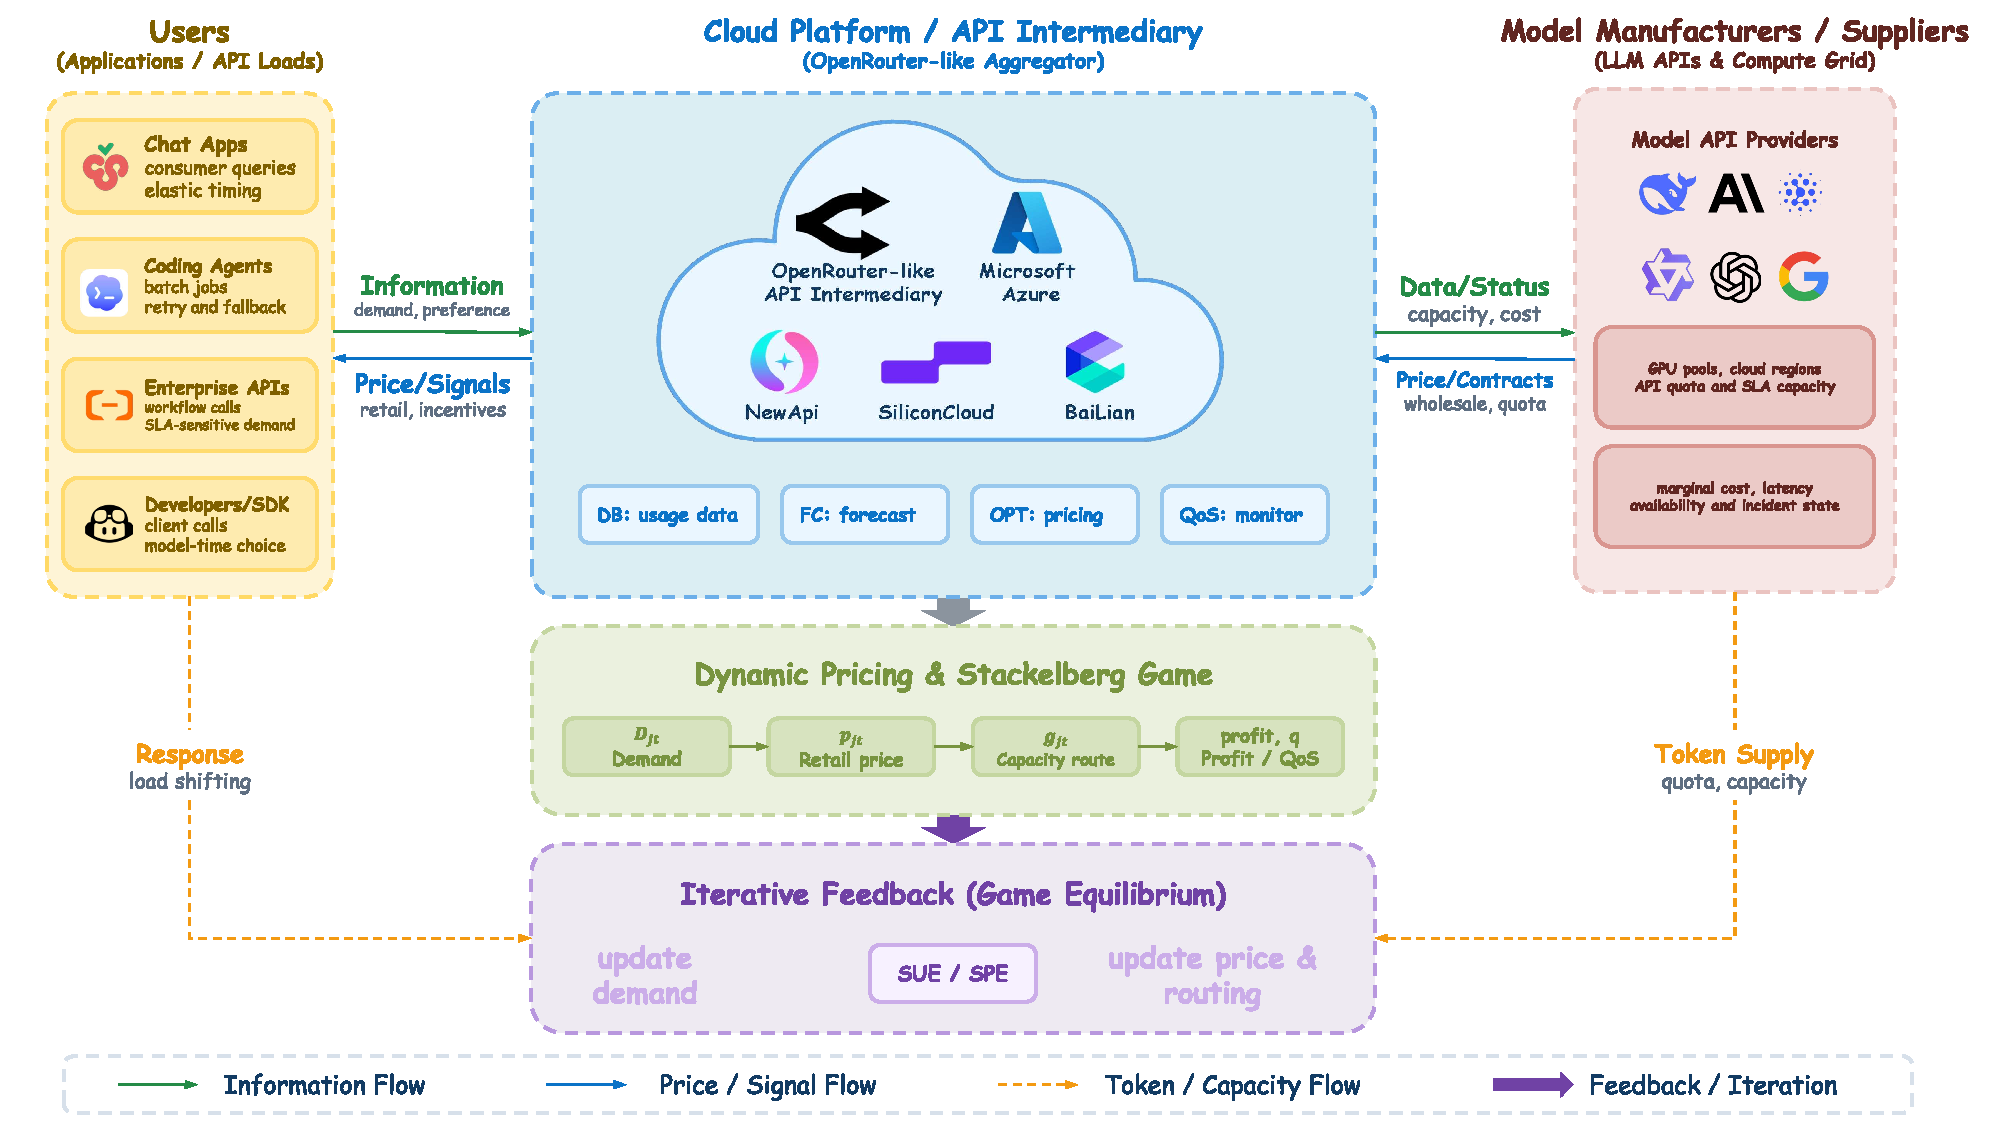
\includegraphics[width=\textwidth]{figures/three_layer_game_framework.pdf}
\caption{平台--中间商--用户三层候选响应框架。}
\label{fig:three_layer_framework}
\end{figure}

% ============================================================
\section{模型哲学与框架分类}
\label{sec:framework_classification}

\subsection{本文模型的本体论定位}

在进入数学模型之前，本节先明确本文框架在博弈论和仿真方法谱系中的精确位置，以避免将算法诱导的计算对象误读为经典均衡理论对象。本文的核心计算结构是一个\textbf{嵌套固定点仿真系统}，由三个异构层组成：

\begin{itemize}[leftmargin=2em]
  \item \textbf{博弈层：} 有限用户的拥塞博弈，通过Rosenthal势函数建立个体层PSNE存在性，为后续聚合选择提供微观理性基础。
  \item \textbf{固定点层：} 连续用户的含退出选项logit SUE与QoS退化构成的复合自映射$q\mapsto\widehat q(q)$，由Brouwer不动点定理保证解的存在性，由阻尼迭代产生实际计算中调用的用户需求和QoS响应。
  \item \textbf{求解器层：} 中间商的最优响应由SLSQP约束优化器在非凸利润曲面上执行局部搜索；平台的最优批发价由有限候选集合内的穷举排序确定。
\end{itemize}

这三层的数学性质截然不同，它们的计算关系是\textbf{嵌套调用}：求解器层在每次目标评估中调用固定点层；固定点层的QoS输入来自求解器层产生的容量和需求；博弈层为固定点层提供从离散到连续的过渡解释，但不是数值计算的直接部件。因此，本文的总体数学对象既不是经典Stackelberg均衡（因为中层响应不是从上层策略到下层策略的单值函数），也不是标准$\epsilon$-Nash均衡（因为偏离检查仅限给定求解器的搜索半径），而是一个\textbf{算法诱导的嵌套固定点候选响应系统（AINF-CRS）}。

\subsection{与经典均衡概念的边界}

表~\ref{tab:framework_vs_classical} 将本文的计算对象与经典博弈论概念做系统对照，用于界定哪些结论可以从数值结果中得出、哪些不能。

\begin{table}[H]
\centering
\caption{本文框架与经典均衡概念的边界对照}
\label{tab:framework_vs_classical}
\small
\begin{tabular}{@{}>{\raggedright\arraybackslash}p{0.20\textwidth}>{\raggedright\arraybackslash}p{0.37\textwidth}>{\raggedright\arraybackslash}p{0.35\textwidth}@{}}
\toprule
经典概念 & 在本文中的状态 & 不能替代的原因 \\
\midrule
Stackelberg均衡 & 仅作为额外正规条件下的\textbf{理论参照系}，不声称数值实例满足这些条件 & 中层响应是求解器诱导的路径依赖输出，不是从$\w$到$(\p,\g)$的单值函数或上半连续对应 \\
\midrule
$\epsilon$-Nash均衡 & 给出\textbf{不可计算的理想参照}；实际报告的$\widehat R_j$只检查SLSQP搜索半径内的偏离 & 全局最优偏离在非凸中层问题中没有求解证书 \\
\midrule
logit SUE & 仅应用于\textbf{用户层}；是唯一具有严格存在性证明和压缩条件下收敛判据的层 & 不适用于中层非合作响应 \\
\midrule
势博弈PSNE & 仅应用于\textbf{离散用户层}；为聚合logit模型提供微观基础 & 枚举$|\A|^N$不可计算，不直接进入数值仿真 \\
\midrule
\textbf{本文计算对象} & \textbf{AINF-CRS}：用户固定点+求解器regret-bounded中层响应+平台候选排序的三层嵌套系统 & 该对象是本文定义的可复核计算实体，不等同于以上任何经典概念 \\
\bottomrule
\end{tabular}
\end{table}

\subsection{什么样的结论可以从AINF-CRS中得出}

在给定求解器$\mathcal{A}$、候选集合$\mathcal{W}_K$和参数化$\theta$下，本文框架可以支持机制诊断（$A$策略相比$B$策略是否产生更高系统利润/QoS/inclusive value，及其价格--容量--拥塞链条）、求解器稳定性（候选响应邻域内是否还能找到超过$\epsilon_N$的单边改进）、候选集合内排序、以及参数敏感性边界。本文框架\textbf{不能}支持的结论包括：连续批发价空间的全局领导者最优性、非凸中层问题的全局Nash均衡证书、跨求解器不变性结论，以及将合成参数下的数值增益直接解释为生产系统的预期利润提升。

% ============================================================
\section{数学模型}
\label{sec:formulation}

设一天被划分为$T$个时段$\T=\{1,\ldots,T\}$，中间商集合为$\J=\{1,\ldots,J\}$。平台发布批发价向量$\w=(w_1,\ldots,w_T)$。中间商$j$为时段$t$分配可服务容量$g_{j,t}\ge \underline g>0$，并发布零售价$p_{j,t}$。服务质量由中间商局部负载决定：
\begin{equation}
  u_{j,t}=\frac{\D_{j,t}}{g_{j,t}},\qquad
  q_{j,t}=\qos(u_{j,t})=
  \begin{cases}
    1, & u_{j,t}\le \bar u,\\
    \exp[-\kappa(u_{j,t}-\bar u)^2], & u_{j,t}>\bar u,
  \end{cases}
  \label{eq:qos}
\end{equation}
其中$\D_{j,t}$是流向中间商$j$在时段$t$的总需求。式~\eqref{eq:qos} 是基准（阈值型）QoS函数；第~\ref{sec:smooth_qos} 节给出线性、Sigmoid和根号三种平滑替代形态的敏感性。

平台收入、中间商利润和系统利润分别为
\begin{align}
  \Pi^P(\w,\p,\g)
  &=h\sum_{j\in\J}\sum_{t\in\T} w_t\D_{j,t}q_{j,t}, \label{eq:platform_profit}\\
  \Pi^I(\w,\p,\g)
  &=h\sum_{j,t}(p_{j,t}-w_t)\D_{j,t}q_{j,t}
    -h\sum_{j,t}c_g g_{j,t}
    -h\sum_{j,t}c_q(1-q_{j,t})\D_{j,t}, \label{eq:intermediary_profit}\\
  \Pi^S(\w,\p,\g)&=\Pi^P+\Pi^I. \label{eq:system_profit}
\end{align}
QoS下降既减少有效结算量，也通过$c_q$表示SLA违约或服务补偿成本。

\subsection{下层模型：含外部退出选项的用户选择}
\label{sec:lower_user}

用户$i$对内部组合$(j,t)$的效用为$U_{i,j,t}=z_{j,t}+\epsilon_{i,j,t}$，其中
\begin{equation}
  z_{j,t}=\log(b_j+\varepsilon)+\log(a_t+\varepsilon)
  -\alpha\left[p_{j,t}+c_s(1-\pi_t)-p_0\right]
  -\gamma[1-q_{j,t}],
  \label{eq:random_utility}
\end{equation}
$\epsilon_{i,j,t}$独立同分布为Gumbel噪声，$\pi_t=\Pr(\tau_i=t)$表示用户原生偏好时段分布，迁移成本项$c_s(1-\pi_t)$是对个体迁移成本$c_s\mathbf{1}[t\ne\tau_i]$的人口期望。

\textbf{外部退出选项（本版关键修正）。} 设一个确定效用为$u_0$（基准取$u_0=0$）的no-purchase外部选项$j=0$。用户在内部选项与退出之间按logit选择：
\begin{equation}
  s_{j,t}=\frac{\exp(z_{j,t})}
  {\exp(u_0)+\sum_{k\in\J}\sum_{\tau\in\T}\exp(z_{k,\tau})},
  \qquad
  s_0=\frac{\exp(u_0)}
  {\exp(u_0)+\sum_{k,\tau}\exp(z_{k,\tau})}.
  \label{eq:logit_share_outside}
\end{equation}
此时内部份额之和$\sum_{j,t}s_{j,t}=1-s_0<1$，残余质量$s_0$为真实退出概率，\textbf{不再}被重新分配回内部选项。这与早期版本的关键区别在于：当价格抬高使$z_{j,t}$普遍下降时，需求会真正流失到退出选项，而不是被softmax归一化掩盖。用户侧inclusive value相应定义为
\begin{equation}
  W^U=\log\!\left[\exp(u_0)+\sum_{j,t}\exp(z_{j,t})\right],
  \label{eq:inclusive_value}
\end{equation}
退出概率$s_0=1/[1+\exp(W^U-u_0)]$与利润评估处于\textbf{同一模型}，从而消除早期版本“利润按零退出计算、退出概率按有退出选项计算”的内部矛盾。当移除退出选项（令$u_0\to-\infty$）时，式~\eqref{eq:logit_share_outside} 退化为早期版本的全内部归一化。

\subsection{需求函数（本版关键修正）}
\label{sec:demand}

给定份额$s_{j,t}$，需求由弹性项和刚性/重放项组成：
\begin{equation}
  \D_{j,t}
  =\underbrace{\bar F\,m(\p)\,s_{j,t}}_{\text{弹性需求}}
  +\underbrace{\bar R_t\,\sigma[\beta(v_r-p_{j,t})]\,s_{j,t}}_{\text{刚性/重放需求（已修正）}},
  \label{eq:demand}
\end{equation}
其中$m(\p)=1+\mu\max(p_0-\bar p_{\mathrm{avg}},0)$为随平均零售价下降而扩张的市场规模因子，$\sigma[\beta(v_r-p_{j,t})]$给出价格超过保留价值$v_r$后的流失比例。

\textbf{与早期版本的差异。} 早期版本刚性项写作$\bar R_t\,\sigma[\beta(v_r-p_{j,t})]\sum_{k\in\J}s_{k,t}$，即对每个中间商$j$都乘以\textbf{整个时段的总份额}$\sum_k s_{k,t}$。对该时段所有中间商求和后得
\[
\sum_{j}\D^{\mathrm{rigid},\text{旧}}_{j,t}
=\bar R_t\Big(\textstyle\sum_k s_{k,t}\Big)\sum_j\sigma[\beta(v_r-p_{j,t})],
\]
其中$\sum_j\sigma(\cdot)$随中间商数量$J$增长——市场里渠道越多，凭空出现的“刚性到达”越多，这与$\bar R_t$应为时段外生请求总量的物理含义矛盾。本版改为按渠道自身份额$s_{j,t}$分配（式~\eqref{eq:demand}），使每时段刚性总量
\[
\sum_{j}\D^{\mathrm{rigid}}_{j,t}=\bar R_t\sum_j s_{j,t}\,\sigma[\beta(v_r-p_{j,t})]
\]
不再随$J$线性放大，且在$J=1$时与早期版本完全一致。第~\ref{sec:simulation_results} 节量化了该修正对所有跨$J$比较的影响。

\subsection{用户层固定点存在性}

logit份额、需求和QoS构成复合自映射$\widehat q:\mathcal{Q}\to\mathcal{Q}$，$\mathcal{Q}=[0,1]^{J\times T}$。

\begin{proposition}[用户层SUE固定点存在性]
\label{prop:sue_fixed_point}
给定任意可行零售价$\p$和正容量$\g$，若需求函数连续、QoS函数连续且取值于$[0,1]$，则联立式~\eqref{eq:logit_share_outside}--\eqref{eq:demand} 与$q_{j,t}=\qos(\D_{j,t}/g_{j,t})$的用户层SUE--QoS固定点至少存在一个。若进一步复合Lipschitz常数$L_\qos L_D L_s<1$，则固定点唯一，阻尼迭代以线性速率收敛。
\end{proposition}

\begin{proof}
对任意$q\in\mathcal{Q}$，式~\eqref{eq:logit_share_outside} 给出连续份额，式~\eqref{eq:demand} 给出连续需求，再给出新QoS向量$\widehat q(q)=\qos(\D/g)$。由于$\qos(\cdot)\in[0,1]$，$\widehat q:\mathcal{Q}\to\mathcal{Q}$是连续自映射，$\mathcal{Q}$非空、紧且凸，由Brouwer不动点定理至少存在$q^*=\widehat q(q^*)$。若复合Lipschitz常数小于1则$\widehat q$为压缩映射，Banach不动点定理给出唯一性和收敛性；阻尼更新$q^{\ell+1}=\eta\widehat q(q^\ell)+(1-\eta)q^\ell$在同一压缩条件下仍为压缩。
\end{proof}

\begin{remark}[退出选项不破坏存在性]
加入退出选项只是把logit归一化分母增加一个正常数$\exp(u_0)$，份额仍连续，故命题~\ref{prop:sue_fixed_point} 的连续自映射结构不变。
\end{remark}

\subsection{有限用户拥塞博弈与微观基础}

用户层的离散对应是有限拥塞博弈。用户$i$选择$(j,t)$的确定性收益含品牌、时段偏好、价格和拥塞负效用项。

\begin{proposition}[用户侧PSNE存在性]
\label{prop:psne}
由有限用户拥塞负效用定义的博弈是精确势博弈，因此存在纯策略Nash均衡。
\end{proposition}

\begin{proof}[证明要点]
构造Rosenthal型势函数，其中拥塞项写为$-\delta\sum_{j,t}\sum_{k=1}^{n_{j,t}}[1-\qos(k/\bar g_{j,t})]$。单边偏离时其余用户项抵消，势函数变化恰等于偏离用户收益变化，故为精确势博弈；有限精确势博弈至少有一个局部最大势配置即为PSNE\cite{rosenthal1973class,monderer1996potential}。
\end{proof}

从有限PSNE到连续logit SUE的过渡是大人口近似，在人口博弈文献中有标准讨论\cite{sandholm2010population}，本文不贡献新的收敛定理。

\subsection{中层模型与算法诱导候选稳定性}
\label{sec:middle_intermediary}

给定$\w$，中间商$j$选择$(\p_j,\g_j)$满足$\sum_t g_{j,t}=G_j$、$g_{j,t}\ge\underline g$、$p_{j,t}\in[\underline p,\overline p]$。其\textbf{算法诱导响应}定义为SLSQP求解器在初值$x_j^{(0)}$下返回的局部最优解$\widehat{\mathcal{BR}}_j(\w,x_{-j};\mathcal{A})$。注意此处“$\arg\max$”只表示求解器返回的局部最优，不是全局最大。

\begin{definition}[算法诱导候选稳定性]
\label{def:solver_regret_candidate}
定义算法诱导regret
\begin{equation}
  \widehat R_j(x;\w;\mathcal{A})=
  \max\!\left\{
  \Pi^I_j(\w,\widehat{\mathcal{BR}}_j(\w,x_{-j};\mathcal{A}),x_{-j})
  -\Pi^I_j(\w,x_j,x_{-j}),\,0
  \right\}.
  \label{eq:solver_reported_regret}
\end{equation}
若$\max_{j\in\J}\widehat R_j\le\epsilon_N$（本文取$\epsilon_N=10^{-3}$），则称$x$满足$\w$下的算法诱导候选稳定性。
\end{definition}

\textbf{语义边界。} $\widehat R_j$是求解器分辨率下的局部偏离诊断，不是标准博弈论的$\epsilon$-Nash regret：它用求解器局部搜索替代了策略空间上的全局最大化，依赖求解器配置$\mathcal{A}$，且不排除搜索半径之外存在更优偏离。后文所有“regret”均指$\widehat R_j$。

\begin{remark}[条件性SPE理论边界]
严格SPE存在需要额外正规条件（用户层响应可选取为连续函数、中间商可行集非空紧凸、$\Pi^I_j$拟凹、中层均衡对应上半连续、平台诱导值函数上半连续）。第~\ref{sec:simulation_results} 节的利润切面诊断显示中层利润函数在容量方向存在多个浅局部峰，这些正规条件在本文合成实例中\textbf{未经验证且可能不成立}，因此本文统一报告算法诱导regret而不声称严格SPE。
\end{remark}


% ============================================================
\section{求解方法}
\label{sec:solution}

\subsection{三层候选响应的迭代计算}
\label{sec:fixed_point}

本算法将用户层含退出选项的logit SUE--QoS固定点迭代嵌入中间商最优响应的内循环，再将中间商响应嵌入平台批发价候选排序的外循环。给定批发价候选$\w\in\mathcal{W}_K$，算法$\mathcal{A}$返回一个由初值、随机种子和求解器路径诱导的中层响应$\widehat x(\w;\mathcal{A})$。平台层执行候选排序
\begin{equation}
  (\widehat\w,\widehat x)\in
  \arg\max_{\w\in\mathcal{W}_K}
  \left\{
  \Pi^P(\w,\widehat x(\w;\mathcal{A})):
  \max_{j}\widehat R_j\le\epsilon_N
  \right\}.
  \label{eq:platform_mapping}
\end{equation}
$\mathcal{W}_K$是启发式批发价候选集合，式~\eqref{eq:platform_mapping} 只定义候选集合内和给定求解路径下的收入排序，不声称解决连续空间上的全局领导者最优问题。平台层连续最优化（贝叶斯优化、多起点梯度、演化策略）作为后续工作方向，本文未实现。

\subsection{算法流程与计算环境}
\label{sec:algorithm}

\begin{table}[H]
\centering
\algcaption{多起点分布式迭代三层候选响应求解}
\label{alg:full_backward}
\begin{tabular}{p{0.96\textwidth}}
\toprule
\textbf{输入：} 平台、中间商和用户参数；候选批数$K$；SLSQP最大迭代$M$；中间商最优响应轮数$B$；阻尼系数$\eta$；容差$\epsilon$；退出选项效用$u_0$。\\
\textbf{输出：} 各策略的批发价、零售价、容量、需求、QoS、利润、inclusive value、退出概率及诊断字段。\\
\midrule
1.\quad 生成$K$个批发价候选：首轮取基准批发价，后续为$[\underline w,\overline w]^T$内随机采样。\\
2.\quad 对每个候选$\w$：初始化中间商策略；对$b=1,\ldots,B$依次为每个中间商调用SLSQP求解给定其他中间商策略时的最优$(\p_j,\g_j)$，每次目标评估内嵌算法~\ref{alg:user_sue_fixpoint}。\\
3.\quad 计算最大solver-based regret，若不超过$\epsilon_N$则接受为候选响应。\\
4.\quad 在已返回候选中选平台收入最高者。\\
5.\quad 对统一零售、单中间商、无QoS动态定价和QoS感知三层定价逐一求解，汇总指标并保存工件。\\
\bottomrule
\end{tabular}
\end{table}

\begin{table}[H]
\centering
\algcaption{用户层含退出选项logit SUE固定点迭代}
\label{alg:user_sue_fixpoint}
\begin{tabular}{p{0.96\textwidth}}
\toprule
\textbf{输入：} 零售价、容量、时段偏好、QoS参数、阻尼$\eta$、容差$\epsilon$、最大迭代$L$、退出效用$u_0$。\\
\midrule
1.\quad 初始化$q_{j,t}\leftarrow1$。\\
2.\quad 对$\ell=1,\ldots,L$：按式~\eqref{eq:random_utility} 算效用$z_{j,t}$；按式~\eqref{eq:logit_share_outside} 含退出选项归一化得份额$s_{j,t}$与退出概率$s_0$；按式~\eqref{eq:demand}（修正口径）算需求；算利用率与目标QoS；若残差$\le\epsilon$返回；否则阻尼更新$q\leftarrow\eta\hat q+(1-\eta)q$。\\
\bottomrule
\end{tabular}
\end{table}

所有仿真在AMD Ryzen 9 9950X、16 GB RAM、WSL2 Linux、Python 3.12环境执行。阻尼系数$\eta=0.35$，容差$\epsilon=10^{-9}$，最大迭代$L=200$，$K=8$，退出效用基准$u_0=0$。

% ============================================================
\section{案例研究}
\label{sec:case_study}

\subsection{实验设置与复现验证}
\label{sec:basic_data}

一天划分为$T=8$个时段（$h=3$小时），中间商数$J=3$。容量预算$G_j=(1050,1080,1080)$，统一零售价$p_0=0.80$，统一批发价$w_0=0.40$，批发价边界$[0.25,0.90]$，零售价边界$[0.45,2.10]$。QoS退化参数$\bar u=0.82,\kappa=15.0$，价格敏感度$\alpha=3.5$，迁移成本$c_s=0.20$，QoS反馈权重$\gamma=1.0$，单位容量成本$c_g=0.015$，单位退化成本$c_q=0.35$。刚性需求基线$(200,150,300,600,800,900,700,250)$，弹性基数$\bar F=400$。所有经济参数均为合成设定。

\textbf{复现验证（修正代码忠实性）。} 本版重写了三层求解管线，并加入需求口径与退出选项的可开关修复。为确保重写忠实于早期实现，在关闭所有修复开关时，重写代码必须重现早期工件的数值。表~\ref{tab:fidelity} 确认四个基线在“开关全关”下逐位重现早期数字（误差$<0.01$），从而保证后续“开关打开”得到的修正数字反映的是修复本身，而非重写引入的差异。

\begin{table}[H]
\centering
\caption{复现验证：关闭所有修复开关时，重写管线重现早期工件数值。}
\label{tab:fidelity}
\begin{tabular}{lrrr}
\toprule
策略 & 重写（开关全关） & 早期工件 & 差 \\
\midrule
统一零售 & 4911.97 & 4911.97 & $-0.00$ \\
单中间商 & 2308.55 & 2308.55 & $+0.00$ \\
无QoS动态定价 & 8383.79 & 8383.79 & $+0.00$ \\
三层QoS感知 & 9525.11 & 9525.12 & $-0.01$ \\
\bottomrule
\end{tabular}
\end{table}

\subsection{修正一：需求口径放大效应的量化}
\label{sec:simulation_results}

表~\ref{tab:fix_baselines} 报告三种设置下五类（含两个共用）基线的系统利润：RAW（开关全关，等于早期版本）、M1（仅修正需求口径放大）、M1+M3（同时加入外部退出选项）。

\begin{table}[H]
\centering
\caption{需求口径修正与外部退出选项对基线结果的影响（系统利润为重跑真实值）。}
\label{tab:fix_baselines}
\small
\resizebox{\textwidth}{!}{%
\begin{tabular}{lrrrr}
\toprule
策略 & RAW（早期口径） & M1（口径修正） & M1+M3（加退出选项） & 说明 \\
\midrule
统一零售 & 4911.97 & 2308.55 & 2136.45 & RAW因$J{=}3$放大 \\
单中间商 & 2308.55 & 2308.55 & 1844.70 & $J{=}1$，M1下不变 \\
无QoS动态定价 & 8383.79 & 3079.24 & 2306.59 & 增量参照 \\
三层QoS感知定价 & 9525.11 & 3089.19 & 2306.59 & 主策略 \\
\bottomrule
\end{tabular}%
}
\end{table}

\textbf{放大效应的直接证据。} 在RAW设置下，统一零售（$J{=}3$）系统利润4911.97是单中间商（$J{=}1$）2308.55的2.13倍；总需求比值为2.19。这一差异曾被解读为“渠道差异化与竞争带来的需求增量”。但修正需求口径后（M1），统一零售$J{=}3$回落到2308.55，与单中间商$J{=}1$\textbf{完全相同}，总需求比值降为1.00。这证明早期“中间商越多系统利润越高”的结论\textbf{主要是需求口径放大的人为产物}，而非真实的渠道经济价值。

\textbf{对QoS感知增益的影响。} 在RAW设置下，三层QoS感知（9525.11）相对无QoS动态（8383.79）的增益为$+13.61\%$。修正口径后（M1），二者分别为3089.19和3079.24，增益降为$\mathbf{+0.32\%}$。原因在第~\ref{sec:conditional_gain} 节解释：去掉放大需求后，原始需求水平下市场并不拥塞，QoS感知缺乏发挥空间。

\subsection{修正二：QoS感知的条件性增益}
\label{sec:conditional_gain}

QoS感知只有在市场真正拥塞、利用率逼近退化阈值时才有价值。为定位这一区间，本文在M1修正口径下对需求规模因子$\rho$做扫描（$\rho$同时缩放刚性与弹性基线）。表~\ref{tab:demand_scale} 给出结果。

\begin{table}[H]
\centering
\caption{需求规模扫描下QoS感知相对无QoS动态定价的条件性增益（M1修正口径，重跑真实值）。}
\label{tab:demand_scale}
\small
\begin{tabular}{rrrrr}
\toprule
需求规模$\rho$ & 无QoS利润 & QoS感知利润 & QoS增益 & 无QoS峰值利用率 \\
\midrule
1.0（原始水平） & 3079.24 & 3089.19 & $+0.32\%$ & 0.852 \\
1.3 & 3594.08 & 4059.28 & $+12.94\%$ & 0.955 \\
1.6 & 4602.13 & 5029.38 & $+9.28\%$ & 0.859 \\
2.0 & 5521.92 & 6322.83 & $+14.50\%$ & 0.902 \\
\bottomrule
\end{tabular}
\end{table}

\textbf{核心发现。} QoS感知的价值是\textbf{条件性的}。在原始需求水平（$\rho=1.0$），无QoS动态定价的峰值利用率仅0.852，市场基本不拥塞，QoS感知几乎无增益（$+0.32\%$）。但当需求升高到$\rho\ge1.3$、无QoS策略的峰值利用率突破0.86--0.96、最低QoS跌到0.76--0.90时，QoS感知通过把容量重新分配并控制临界利用率，重新获得$+9.3\%$至$+14.5\%$的真实系统利润改善，并在所有这些场景下把最低QoS恢复到1.0000。这一修正后的结论比早期的无条件$+13.61\%$更可信、更可证伪：它明确指出QoS感知定价的适用边界是\textbf{拥塞区间}，并给出该边界的需求规模阈值。

\subsection{修正三：平滑QoS形态与相位锁定诊断}
\label{sec:smooth_qos}

早期版本报告“最低QoS=1.0000、峰值利用率精确=0.8200”，这一“完美”结果引发对阈值型QoS函数是否诱导人为边界的质疑。本节补全早期承诺但缺失的平滑QoS形态实验：在M1修正口径下，用三种平滑退化函数替换式~\eqref{eq:qos}，重跑三层QoS感知策略。

\begin{table}[H]
\centering
\caption{QoS函数形态敏感性（M1修正口径，重跑真实值）。峰值利用率随形态显著变化，证实阈值型函数诱导相位锁定。}
\label{tab:smooth_qos}
\small
\begin{tabular}{lrrr}
\toprule
QoS形态 & 系统利润 & 峰值利用率 & 活跃最低QoS \\
\midrule
阈值型（基准，$\exp[-\kappa(u-\bar u)^2]$） & 3089.19 & 0.8105 & 1.0000 \\
线性退化（$u>0.5$起连续下降） & 3089.19 & 0.4994 & 1.0000 \\
Sigmoid平滑（$\kappa_s=30$） & 3089.22 & 0.3764 & 1.0000 \\
根号退化（$\kappa_r=2.5$） & 2813.68 & 0.8086 & 0.9163 \\
\bottomrule
\end{tabular}
\end{table}

\textbf{诊断结论。} 系统利润在阈值、线性、Sigmoid三种形态下高度一致（3089.19--3089.22），说明\textbf{“拥塞风险内化”这一核心机制对QoS函数形态具有方向鲁棒性}。但峰值利用率随形态从0.81剧烈变化到0.38--0.50，这\textbf{证实}早期版本“峰值利用率精确锁定在阈值0.82”确实是阈值型函数“平坦区→尖锐拐点”二阶段结构诱导的\textbf{相位锁定现象}，而非一般性均衡性质。一旦换用退化从低利用率即连续启动的平滑形态，中间商不再有动机把利用率精确顶到某个阈值，峰值利用率自然下移。根号退化（凸型、退化在阈值以上以递减速率增长）下系统利润略低（2813.68）且活跃最低QoS降到0.9163，说明退化曲率方向会影响结果幅度，但不改变利润提升的方向。因此，凡涉及具体峰值利用率数字的结论，都应限定为\textbf{阈值型QoS场景}；而“拥塞内化提升利润、改善QoS底线”的方向性结论对平滑形态稳健。

\subsection{修正四：收入最大化与用户体验的可解释双赢区域}
\label{sec:welfare}

早期版本报告三层QoS感知策略将inclusive value从2.10压低到$-0.52$、退出概率升到62.69\%，并将其作为“收入最大化必然牺牲用户福利”的张力列为局限。但该结论建立在“利润按零退出算、退出概率按有退出选项算”的内部矛盾之上。本节在加入外部退出选项的自洽模型（M1+M3）中重新检验这一张力。

\begin{table}[H]
\centering
\caption{自洽模型（M1+M3，含退出选项）下的收入最大化与价格保护对比（重跑真实值）。}
\label{tab:welfare}
\small
\resizebox{\textwidth}{!}{%
\begin{tabular}{lrrrrr}
\toprule
策略 & 系统利润 & 平台收入 & 平均零售价 & Inclusive value & 退出概率 \\
\midrule
无约束收入最大化 & 2306.59 & 1501.47 & 1.068 & $+1.574$ & 20.7\% \\
价格保护（零售$\le0.80$） & 2104.56 & \textbf{1920.71} & 0.777 & $\mathbf{+2.281}$ & \textbf{10.2\%} \\
\bottomrule
\end{tabular}%
}
\end{table}

\textbf{修正后的两点发现。} 第一，\textbf{自洽模型消除了早期的极端福利崩溃}。加入退出选项后，无约束收入最大化的均衡平均零售价被\textbf{内生约束}在1.068（而非早期失真的1.67），因为继续涨价会触发用户真实退出，反而损害平台收入；相应地inclusive value保持正值$+1.574$，退出概率为20.7\%，而非早期的$-0.52$和62.69\%。这说明早期“福利崩溃”很大程度上是缺少退出选项导致优化器可以无代价抬价的建模假象。

第二，\textbf{价格保护合约形成可解释的双赢区域}。在零售价不超过0.80的保护合约下，平台收入不降反升（从1501.47提高到1920.71），同时inclusive value提高到2.281、退出概率降到10.2\%。其机制是：在含退出选项的市场中，过高的零售价会把大量用户推向退出，无约束优化反而损失了本可结算的需求；价格保护强制平台留在用户愿意参与的价格区间，扩大了实际成交量，因此对平台收入和用户福利同时有利。这是一个比早期“必然牺牲福利”更具政策含义的正面结论：\textbf{在用户拥有外部选项的推理服务市场，适度价格保护可能同时改善平台收入与用户体验}。

\subsection{跨层比较的口径修正}
\label{sec:cross_layer}

早期版本以“二层集中优化4519.28 vs 三层QoS感知9525.12”作为架构对比。本文发现这一对比的两条管线使用了不同的需求口径：三层管线带$J$放大，二层管线不带；二层基准在数值上恰好退化为单中间商结果。因此该对比反映的是需求口径差异而非架构差异。在统一需求口径后，跨层比较应重新进行，且应同时控制市场层级、用户选择集合和定价自由度的变化。本文把跨层架构比较移出主要量化贡献，仅作为方法学注记：去掉中间商层会同时改变用户选择集合、品牌差异和定价自由度，单一系统利润数字不足以支撑一般福利排序。

\subsection{机制归因与解释边界}
\label{sec:discussion}

综合修正后的实验，本文的机制结论可总结为：在推理服务存在可迁移负载和显式QoS退化反馈、\textbf{且市场处于拥塞区间}时，平台通过候选批发价排序可以引导下游容量分配和零售定价，提高系统利润并改善QoS底线。这一增益的核心驱动是\textbf{将拥塞风险内化到中间商决策}——无论通过精确QoS成本还是平滑退化形态表示（第~\ref{sec:smooth_qos} 节）。在非拥塞区间，该机制几乎不产生增益（第~\ref{sec:conditional_gain} 节）。

\textbf{局限与注意事项。} 第一，所有经济参数为合成设定，不能直接解释为真实用户弹性；本文结论是机制层面的方向性发现，不是任意参数下的福利定理。第二，平台层只在有限候选集合内排序，不提供连续批发价空间的领导者最优性证书；多起点检查只检验同一SLSQP求解器的初值敏感性，未建立跨求解器不变性。第三，本文只研究单平台结构。真实推理服务市场存在多个模型厂家，平台间批发价竞争会给上游价格带来下行压力，中间商也可能通过模型切换、路由替代来响应单平台涨价；这些机制会削弱单平台模型中的批发定价权，是本文外部效度的主要限制，需独立建模。第四，外部退出选项的效用$u_0$和价格保护阈值仍是合成设定，真实退出行为需用留存与转化数据校准。第五，凡涉及具体峰值利用率数字的结论限定于阈值型QoS场景。第六，迁移成本在logit聚合层被写成人口期望$c_s(1-\pi_t)$，会压缩原生时段异质性。


% ============================================================
\section{结论}
\label{sec:conclusion}

本文将推理服务的时段性拥塞问题建模为平台--中间商--用户三方分层市场，提出\textbf{算法诱导嵌套固定点候选响应系统（AINF-CRS）}——一个由博弈层（有限PSNE微观基础）、固定点层（含退出选项的logit SUE--QoS自映射）和求解器层（SLSQP局部搜索+候选排序）嵌套构成的离线仿真与机制诊断框架。该框架明确定义了算法诱导候选稳定性判据，并与标准$\epsilon$-Nash和全局SPE做系统性边界划分，定位为离线机制仿真器与策略筛选工具，不声称连续策略空间中的全局均衡证书。

本修订版的核心价值在于：通过修正两处会显著改变定量结论的建模缺陷（需求随中间商数量放大、缺少外部退出选项）并据此重跑全部实验，给出了比早期版本更可信、更可证伪的机制结论：

\textbf{第一，QoS感知定价的增益是条件性的。} 修正需求口径后，原始需求水平下市场并不拥塞，QoS感知仅带来$+0.32\%$增益；早期报告的$+13.61\%$主要是需求放大的人为效应。但当需求升高、利用率逼近容量边界（$\rho\ge1.3$）时，QoS感知恢复$+9.3\%$至$+14.5\%$的真实增益。QoS感知定价的适用边界是拥塞区间。

\textbf{第二，核心驱动是拥塞风险内化，对QoS函数形态鲁棒。} 阈值、线性、Sigmoid三种退化形态下系统利润高度一致；但峰值利用率随形态从0.81变化到0.38--0.50，证实早期“峰值利用率精确=0.82”是阈值函数诱导的相位锁定，而非一般均衡性质。

\textbf{第三，价格保护可形成可解释的双赢区域。} 在含退出选项的自洽模型中，无约束收入最大化的价格被内生约束（平均零售价1.07，inclusive value保持正值$+1.57$）；零售价不超过0.80的价格保护合约同时提高平台收入（1501→1921）、提升inclusive value（1.57→2.28）并降低退出概率（20.7\%→10.2\%）。

在上述严格划定的边界内，本文框架为推理服务平台运营商提供了一种系统的批发定价策略离线筛选方法。未来工作将向四个方向扩展：（一）加入跨求解器不变性诊断；（二）平台层从候选排序升级为贝叶斯优化或演化策略；（三）引入多平台竞争、模型切换和长期容量合约；（四）使用真实生产请求轨迹和用户级弹性估计替代合成参数，实现trace-driven校准和线上A/B验证。

% ============================================================
\section{代码与工件可用性}
\label{sec:code_availability}

匿名审稿材料包含三方市场实验代码、修复版仿真模块、机器可读记录和论文图表。主要工件如下：
\begingroup
\raggedright
\begin{itemize}[leftmargin=2em]
  \item 修复版三层仿真模块（含需求口径与退出选项的可开关修复）：\path{pricing_sim/fixed_market.py}。
  \item 原始（未修正）三层仿真：\path{pricing_sim/intermediary_market.py}、\path{pricing_sim/three_stage_game.py}。
  \item 修正实验入口：\path{experiments/run_reviewer_fixed_experiments.py}（基线RAW/M1/M1+M3、平滑QoS形态）、\path{experiments/run_reviewer_fixed_regime.py}（需求规模扫描、福利张力）。
  \item 复现验证：修复模块在开关全关时重现早期工件数值（表~\ref{tab:fidelity}），保证修正数字反映修复本身。
  \item 修正实验工件：\path{artifacts/reviewer_fixed/20260618/}，含 \texttt{reviewer\_fixed\_records.json}（基线与平滑QoS）、\texttt{demand\_scale\_M1.json}（需求扫描）、\texttt{welfare\_M1\_M3.json}（福利张力）。
  \item 原始实验工件（对照）：\path{artifacts/intermediary/20260608-144953/}。
\end{itemize}
\endgroup
所有修订后数值均可由上述脚本重跑复现；正文每个数字均对应一条落盘的JSON记录。

\small
\bibliographystyle{unsrtnat}
\bibliography{verified_refs}

\end{document}
